\documentclass[11pt]{amsart}
\usepackage{geometry}                % See geometry.pdf to learn the layout options. There are lots.
\geometry{letterpaper}                   % ... or a4paper or a5paper or ... 
%\geometry{landscape}                % Activate for for rotated page geometry
%\usepackage[parfill]{parskip}    % Activate to begin paragraphs with an empty line rather than an indent
\usepackage{graphicx}
\usepackage{amssymb}
\usepackage{epstopdf}
\usepackage[usenames,dvipsnames]{color}
\usepackage{fancyvrb}
\usepackage{listings}
\usepackage{booktabs,footmisc}
\usepackage{hyperref}
\usepackage[all]{hypcap}

\usepackage{topcapt}
\usepackage{enumerate}
\usepackage[section] {placeins}

 
% include the lines below to use a nicer fixed-width font than the default one
 
\lstset{fancyvrb=true}
\lstset{
	basicstyle=\small\tt,
	identifierstyle=,
	commentstyle=\color{Bittersweet},
	stringstyle=\color{red},
	showstringspaces=false,
	tabsize=3,
	numbers=left,
	captionpos=b,
	xleftmargin=2em
%	numberstyle=\tiny
	%stepnumber=4
	}
\DeclareGraphicsRule{.tif}{png}{.png}{`convert #1 `dirname #1`/`basename #1 .tif`.png}

\title{Repast Parameter Sweeps Getting Started}
\author{Mark Bragen \& Mark Altaweel}
%\date{\today}                                           % Activate to display a given date or no date

\begin{document} 
\maketitle

\section{Parameter Sweeps}
The Repast Simphony User Interface has been extended to provide a mechanism for creating parameter sweep and optimized sweep definition files. These definition files can then be submitted for execution on the local computer. Fig.~\ref{fig:sweep1}  is a screen capture of the Parameter Sweep window for the Predator Prey Model.\\

\begin{figure}[h]
\begin{center}
\vspace{.2in}
\centerline {
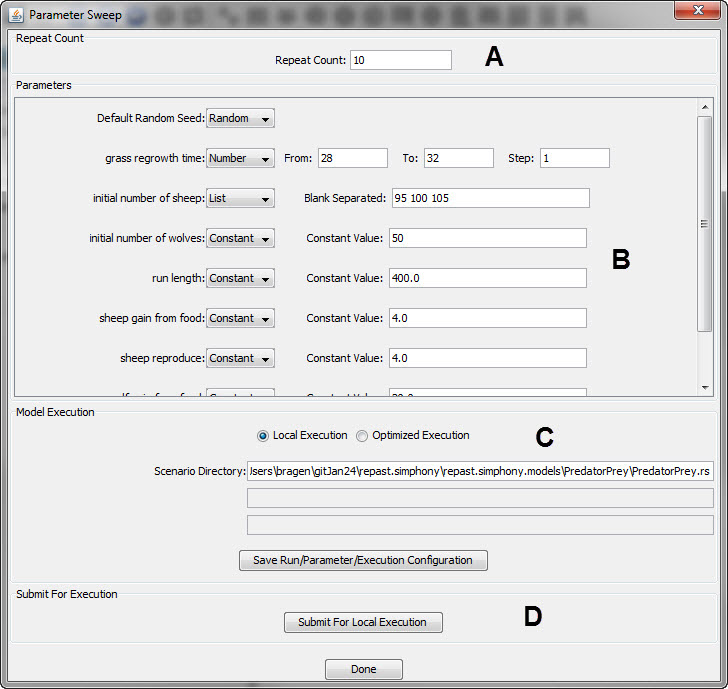
\includegraphics{images/Sweep1.jpg}
}
\caption{}
\label{fig:sweep1}
\end{center}
\end{figure}

The window is divided into four sections:
\begin{enumerate}[ (A) ]
\item Specify the repeat count for the sweep
\item Specify the parameter value definitions for a single sweep
\item Specify the require file information based on execution mode
\item Run submission
\end{enumerate}
\vspace{.2in}

In Section A (see Fig. ~\ref{fig:sweep2} ), the user specifies the number of times that the parameter sweep definitions from Section B will be executed. Note that the parameter sweep definition in Section B specifies a single unit of work that will be executed (i.e. multiple model executions with varying parameter values).\\

\begin{figure}[h]
\begin{center}
\vspace{.2in}
\centerline {
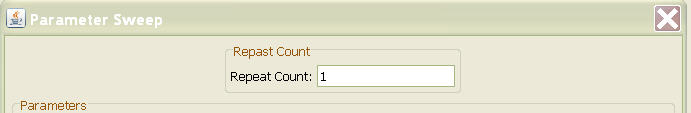
\includegraphics{images/sweep2.jpg}
}
\caption{}
\label{fig:sweep2}
\end{center}
\end{figure}

In Section B (Fig. ~\ref{fig:sweep3}), the user specifies the values for each of the model parameters. Except for the Default Random Seed value, the value(s) can be specified in one of three ways:

\begin{enumerate}
\item A constant value 
\item A list of blank separated values
\item A list of values specified with from, to, step definition
\end{enumerate}
\vspace{.2in}

\begin{figure}[h]
\begin{center}
\vspace{.2in}
\centerline {
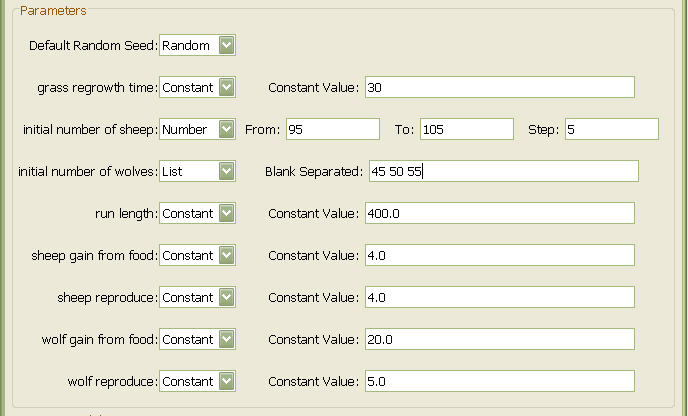
\includegraphics{images/sweep3.jpg}
}
\caption{}
\label{fig:sweep3}
\end{center}
\end{figure}


These are selected from the drop-down selection. Values must be specified for all model parameters. The Default Random Seed has an additional option of a completely random specification. The Random Seed will be determined during the execution of the model.\\

The current settings of the parameters as they appear in Section B, other values that may have been assigned to the parameters for a different specification type (i.e. Constant, List, Number), execution mode, and specified arguments are stored a file in the scenario scenario directory named sweepValues.properties. If this file exists when the Parameter Sweep Window is instaniated, the values stored in the file are extracted and are used to initialize the settings in Section B. If the file does not exist, it is created using the default values as specified in the parameters.xml file. Values will be written to this file only when the "Save Run/Parameter/Execution Configuration" button is clicked or when the "Subment for Execution" button is clicked. Changing a value and then exiting the window via the "Done" button will not update the file.\\


In Section C, the user specifies the type of execution. Two types, each of which has different information requirements, are available:
\begin{enumerate}
\item Local Execution � Execution of the model on the local machine
\item Optimized Execution � Execution of the model on the local machine using a specified optimizer
\end{enumerate}
\vspace{.2in}

In Local Execution mode, the user simply needs to specify the Scenario Directory (see Fig. ~\ref{fig:sweep4a}). Note that this text field is filled by using the scenario directory provided as an argument to the launcher.\\

\begin{figure}[h]
\begin{center}
\vspace{.2in}
\centerline {
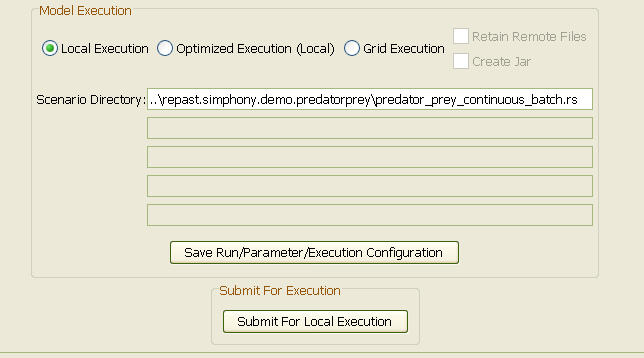
\includegraphics{images/sweep4a.jpg}
}
\caption{}
\label{fig:sweep4a}
\end{center}
\end{figure}

In Optimized Execution mode, the user must specify the Run Result Producer and the Advancement Chooser in addition to the Scenario Directory (see Fig. ~\ref{fig:sweep4b}). Please reference the definitions of these two items in the batch processing documentation.\\

\begin{figure}[h]
\begin{center}
\vspace{.2in}
\centerline {
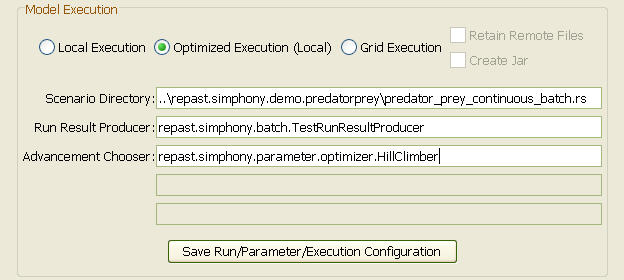
\includegraphics{images/sweep4b.jpg}
}
\caption{}
\label{fig:sweep4b}
\end{center}
\end{figure}



Finally, Section D (see Fig. ~\ref{fig:sweep4a} and ~\ref{fig:sweep4b}) contains the button that will submit the job(s) for execution in one of the three modes. Note that the button text will reflect the execution mode that has been selected in Section C.\\



When the parameter sweep job has been submitted for execution, a console log window will open and display any messages written to stdout from the model execution. See  Fig. ~\ref{fig:sweep6} for an example of this window.


\begin{figure}[h]
\begin{center}
\vspace{.2in}
\centerline {
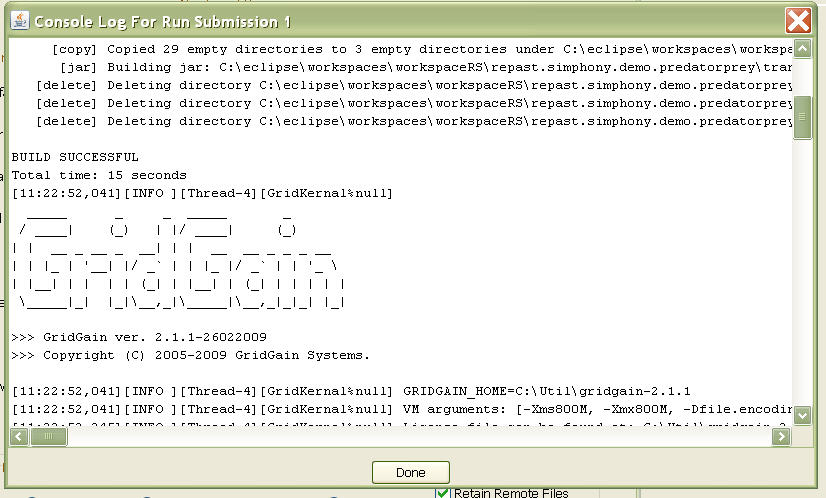
\includegraphics{images/sweep6.jpg}
}
\caption{}
\label{fig:sweep6}
\end{center}
\end{figure}


\end{document}
